\newpage
\begin{center}
    \Huge{\textbf{\underline{Chapter 3: MVC \& PAC}}}
\end{center}

\setcounter{section}{0}

\vspace{0.3cm}


\section{Architectural Design Pattern}
\begin{prettyBox}{Architectural}{myblue}
So far, we’ve only seen the Gang of Four design patterns, which help to implement parts of a project.  
Architectural design patterns such as MVC and PAC structure the entire project by applying the patterns we’ve previously learned.
\end{prettyBox}

\vspace{0.2cm}

\section{Some Terminologies}
\begin{prettyBox}{Definitions}{myblue}
Before explaining MVC and PAC, it is important to understand the following terms:
\begin{itemize}
    \item \textbf{Model (Abstraction)}: the application’s internal data and processing logic.
    \item \textbf{View (Presentation)}: what the user sees and interacts with (Interface).
    \item \textbf{Controller}: the event handler that mediates between the Model and the View.
\end{itemize}
\end{prettyBox}

\vspace{0.2cm}
\section{MVC \& Pac}

\subsection{MVC}
\begin{prettyBox}{MVC (Model View Controller)}{myblue}
The MVC divides the project into 3 categories: Model, View and Controller, but it also imposes how 
these parts interact with each other. It has a circular communication:
\begin{enumerate}
    \item User interacts with the View (interface).
    \item The View sends the user’s request to the appropriate Controller.
    \item Controller changes the Model accordingly.
    \item Model notifies the View.
    \item View updates.
\end{enumerate}
\end{prettyBox}

\vspace{0.1cm}
\begin{center}
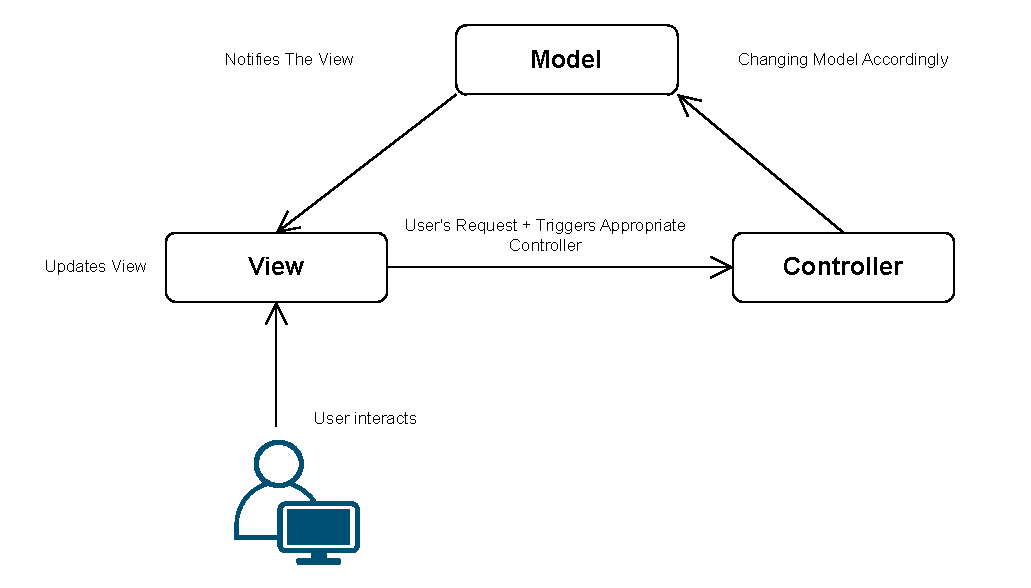
\includegraphics[height=0.25\textheight]{Chapters/MVC_PAC/mvc1.drawio.pdf}
\end{center}

\subsection{PAC}
\begin{prettyBox}{PAC (Presentation Abstraction Controller)}{myblue}
The PAC divides the project into 3 categories: Abstraction (Model), Presentation (View) and Controller, but it also imposes how 
these parts interact with each other. It has a linear communication:
\begin{enumerate}
    \item User interacts with the View (interface).
    \item The View sends the user’s request to the appropriate Controller.
    \item Controller changes the Model accordingly.
    \item Model notifies the Controller.
    \item Controller notifies the View.
    \item View updates.
\end{enumerate}   
\end{prettyBox}

\vspace{0.1cm}
\begin{center}
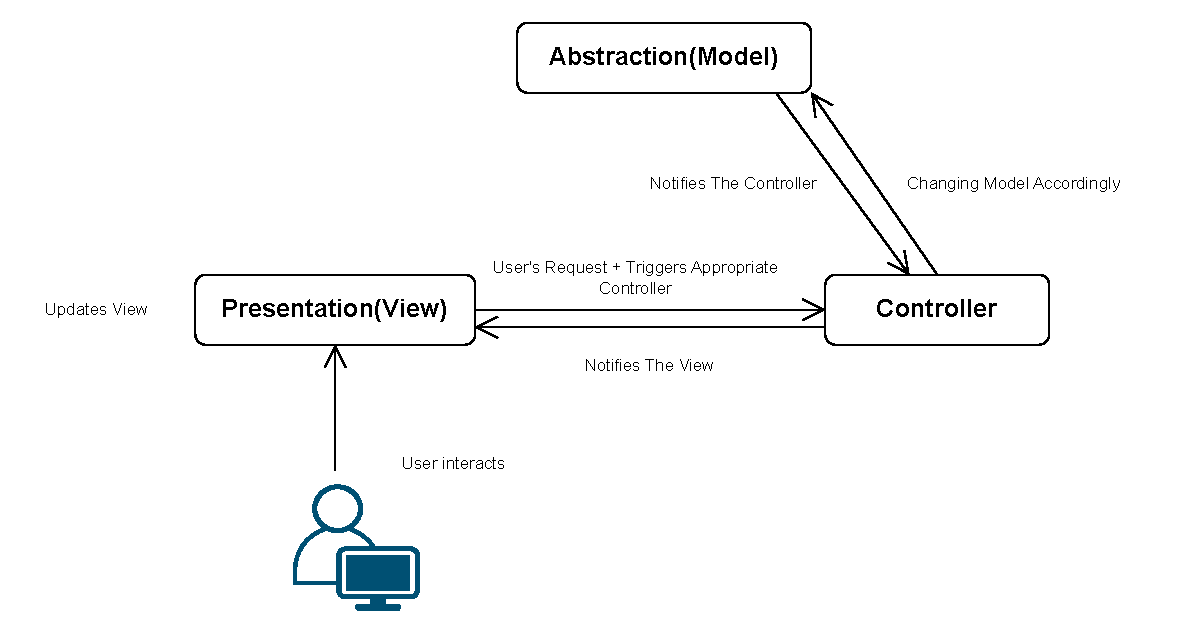
\includegraphics[height=0.25\textheight]{Chapters/MVC_PAC/pac1.drawio.pdf}
\end{center}

\vspace{0.25cm}

\begin{prettyBox}{Note}{red}
Just dividing a project into Model, View and Controller isn't enough to say that it follows MVC or PAC. The way these parts communicate is important too.
\end{prettyBox}

\vspace{0.5cm}

\subsection{Difference Between MVC \& PAC}
\begin{prettyBox}{Difference}{red}
Even though both divide the project into three parts, they differ in how these parts communicate. At first they work
the same: the user interacts with the View, which sends the request to the Controller, which changes the Model. Then they
differ. In MVC, the Model notifies the View directly, creating a circular flow. In PAC, the Model notifies the
Controller, which then notifies the View, creating a linear flow.
\end{prettyBox}

\newpage
\subsection{UML}
\subsubsection{MVC}

\vspace{0.25cm}
\begin{center}
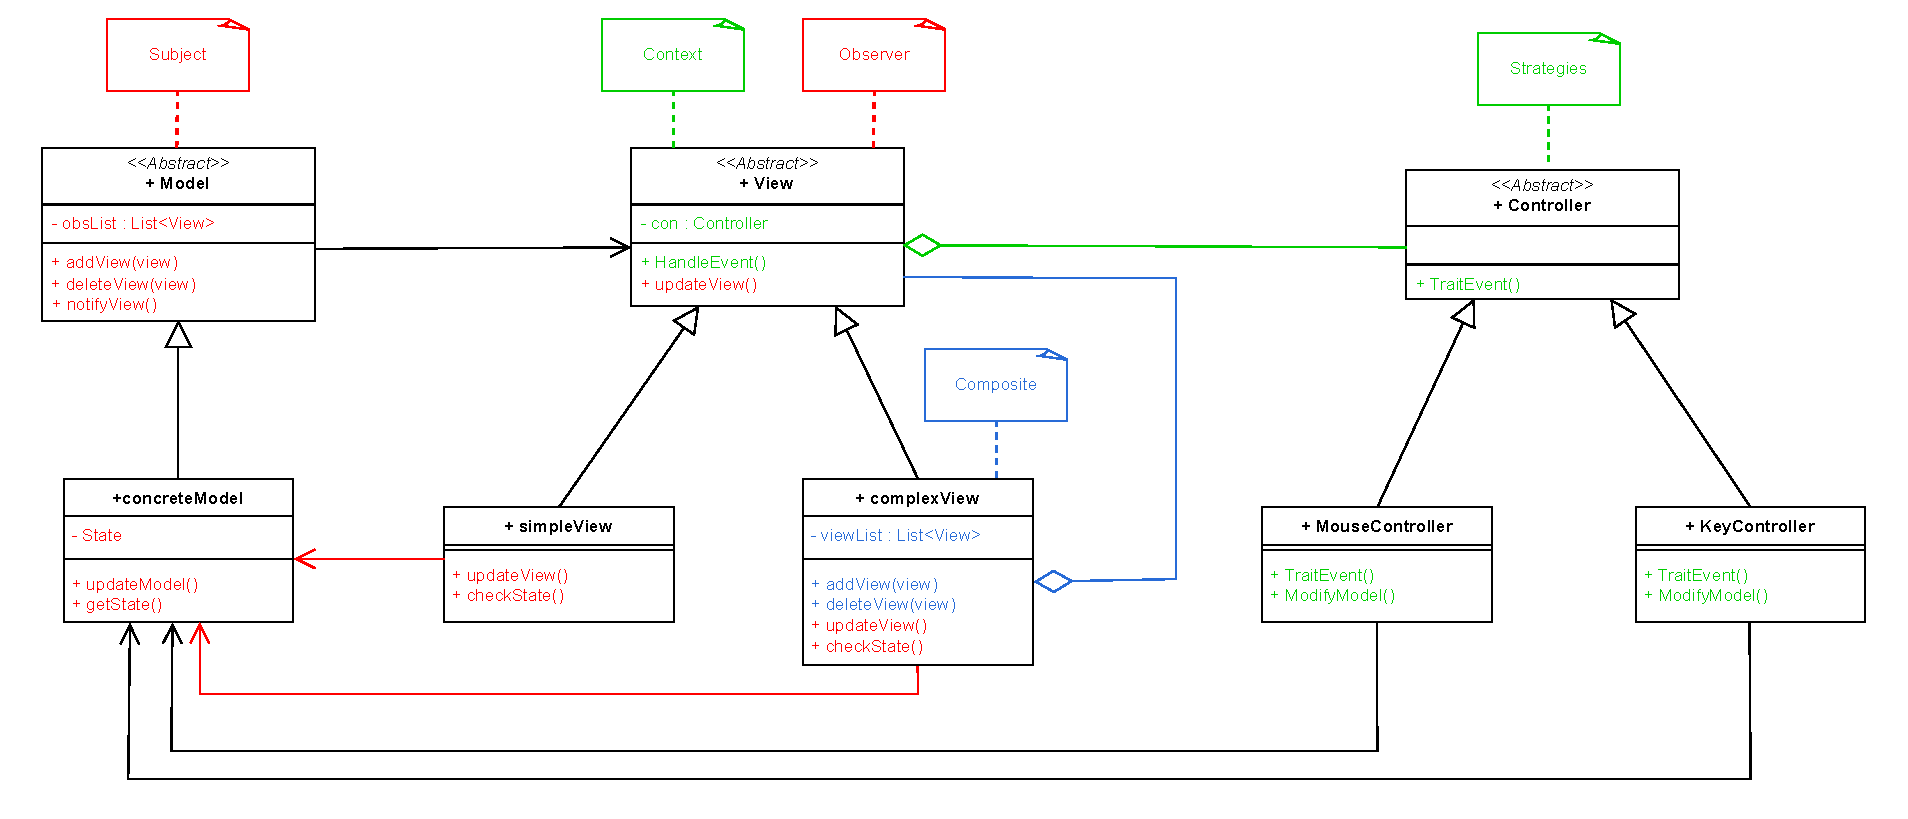
\includegraphics[height=0.25\textheight]{Chapters/MVC_PAC/mvc2.drawio.pdf}
\end{center}

\vspace{0.25cm}


\begin{prettyBox}{Explication}{myblue}
The View uses the Composite design pattern to organize views into a hierarchy of simple and nested views.\\[0.15cm]
The user sees and interacts only with the View, triggering events at runtime, so we apply the Strategy design
pattern between the View and Controller: the View is the context, holds a reference to the Controller, and defines
a \texttt{handleEvent()} method that calls the Controller’s \texttt{traitEvent()}, while each Controller implements
a strategy to update the Model based on the user event. Inside \texttt{traitEvent()} \texttt{modifyModel()} is called and invokes
the Model’s \texttt{updateModel()} method.\\[0.15cm]
We use the Observer design pattern between the Model and View because the Model holds data that external classes
(views) are interested in and that can change at runtime. When \texttt{updateModel()} is called, it runs \texttt{notifyView()},
which loops through all observers(views) of \texttt{obsList} and calls each observer’s \texttt{updateView()} which uses \texttt{getState()}.
\end{prettyBox}

\newpage
\subsubsection{PAC}

\vspace{0.25cm}
\begin{center}
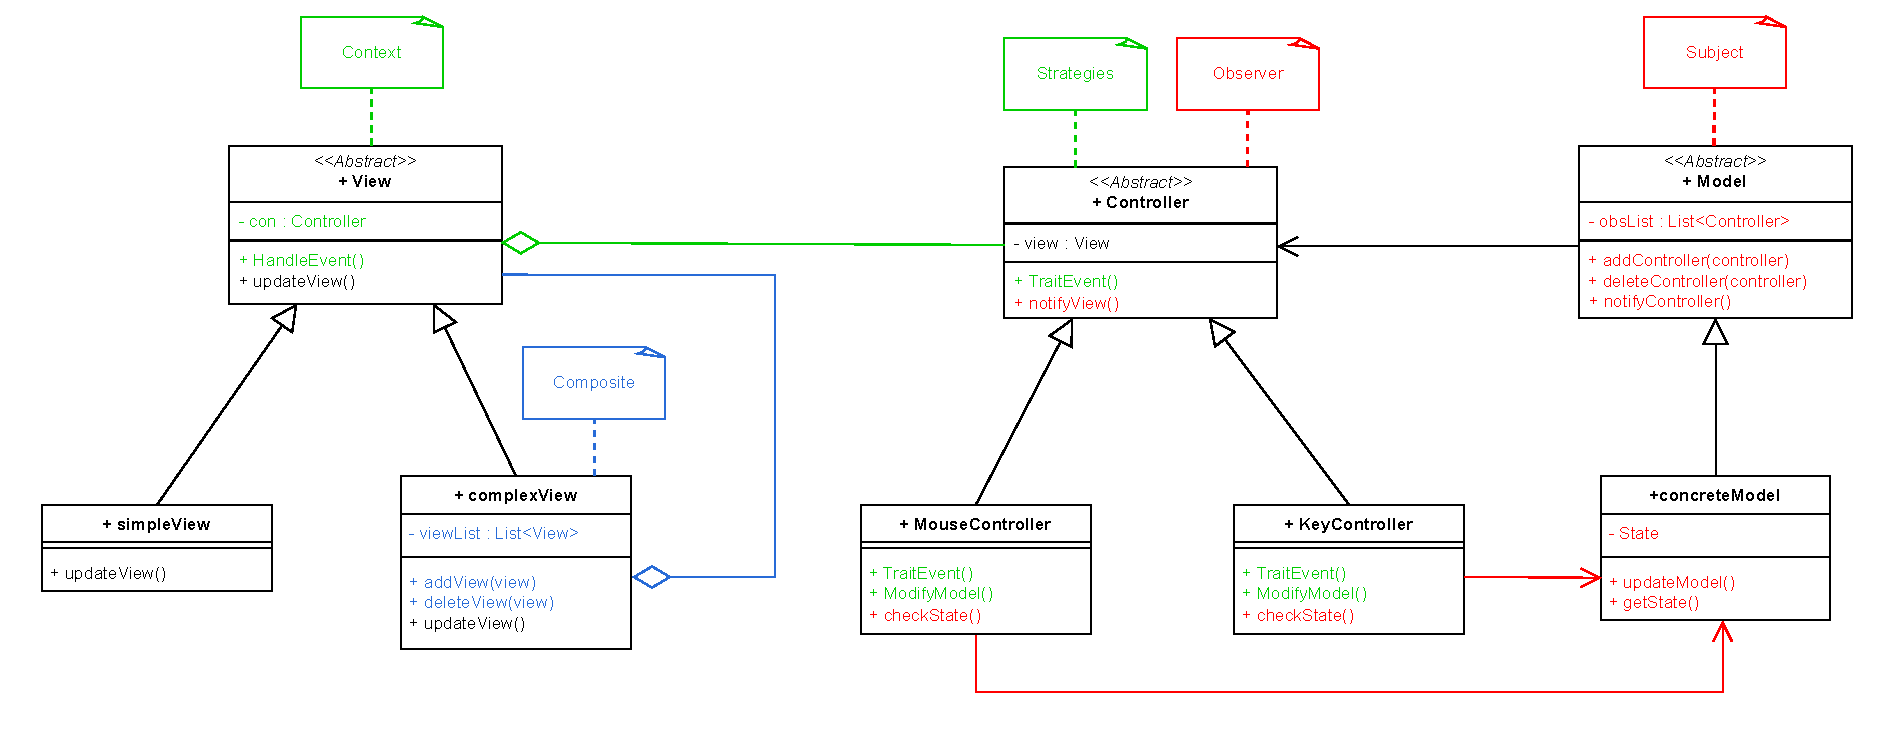
\includegraphics[height=0.25\textheight]{Chapters/MVC_PAC/pac2.drawio.pdf}
\end{center}

\vspace{0.25cm}
\begin{prettyBox}{Explication}{myblue}
The View uses the Composite design pattern to organize views into a hierarchy of simple and nested views.\\[0.15cm]
The user sees and interacts only with the View, triggering events at runtime, so we apply the Strategy design
pattern between the View and Controller: the View is the context, holds a reference to the Controller, and defines
a \texttt{handleEvent()} method that calls the Controller’s \texttt{traitEvent()}, while each Controller implements
a strategy to update the Model based on the user event. Inside \texttt{traitEvent()} \texttt{modifyModel()} is called and invokes
the Model’s \texttt{updateModel()} method.\\[0.15cm]
We use the Observer design pattern between the Model and controller because the Model holds data that external classes
(controller) are interested in and that can change at runtime. When \texttt{updateModel()} is called, it runs \texttt{notifycontroller()} 
which loops through all observers(controllers) of \texttt{obsList} and calls each observer’s \texttt{notifyView()} which calls 
the getstate method , the updateview of the view object held in controller class.
\end{prettyBox}


